\documentclass[11pt,a4paper]{article}
\usepackage[T1]{fontenc}
\usepackage[utf8]{inputenc}
\usepackage{lmodern}
\usepackage[margin=22mm,headheight=16pt]{geometry}
\usepackage{amsmath,amssymb,graphicx,array,longtable,booktabs}
\usepackage{microtype,xcolor,hyperref,xurl,fancyhdr}
\definecolor{Navy}{HTML}{17324D}
\definecolor{Teal}{HTML}{087F8C}
\definecolor{Gold}{HTML}{B88128}
\hypersetup{colorlinks=true,linkcolor=Navy,urlcolor=Teal,bookmarksnumbered=true,hypertexnames=false}
\setlength{\parindent}{0pt}
\setlength{\parskip}{6pt}
\setlength{\emergencystretch}{4em}
\setcounter{tocdepth}{1}
\pagestyle{fancy}\fancyhf{}
\fancyfoot[R]{\small\thepage}
\fancyfoot[L]{\small\sffamily Sharif University of Technology}
\renewcommand{\headrulewidth}{0.3pt}
\makeatletter
\renewcommand\section{\@startsection{section}{1}{\z@}{-3.2ex plus -1ex minus -.2ex}{1.6ex plus .2ex}{\normalfont\Large\sffamily\bfseries\color{Navy}}}
\renewcommand\subsection{\@startsection{subsection}{2}{\z@}{-2.5ex plus -1ex minus -.2ex}{1.2ex plus .2ex}{\normalfont\large\sffamily\bfseries\color{Teal}}}
\makeatother
\fancyhead[L]{\small\sffamily\color{Navy}Sharif University of Technology}\fancyhead[R]{\small\sffamily\color{Teal}Project Assignment}\begin{document}
\begin{titlepage}\centering\vspace*{7mm}

\includegraphics[width=31mm]{assets/sharif_emblem_en.png}\par\vspace{5mm}
{\Large\sffamily\bfseries\color{Navy}SHARIF UNIVERSITY OF TECHNOLOGY\par}
\vspace{2mm}{\sffamily Department of Electrical Engineering\par}
\vspace{17mm}{\color{Teal}\rule{\linewidth}{1.4pt}}\par\vspace{6mm}
{\large\sffamily\color{Teal}PROJECT ASSIGNMENT\par}
\vspace{8mm}{\huge\sffamily\bfseries\color{Navy}MIDI Digital Synthesizer and Audio Effects Prototype\par}
\vspace{9mm}{\color{Gold}\rule{45mm}{1pt}}\par\vfill
\begin{minipage}{.88\linewidth}
{\sffamily\color{Teal}INSTRUCTOR / INSTRUCTORS}\par
Dr Mojahedian\par\vspace{7mm}
{\sffamily\color{Teal}ACADEMIC CONTEXT}\par
Signals and Systems\par\end{minipage}\vfill
\end{titlepage}
\tableofcontents\clearpage
\section{Deliverables and assessment}

Build a MIDI-to-audio synthesizer followed by a configurable series of audio effects, using Python or MATLAB. Package source, report, figures, and audio outputs together. The original naming convention is Project-StudentNo1\_\allowbreak{}StudentNo2\_\allowbreak{}StudentNo3.zip. Supply the report PDF and its LaTeX source when using LaTeX. The course submission requires a GitHub repository. The grading table assigns synthesis 0.45 plus 0.1 bonus, GitHub 0.05, LaTeX/\allowbreak{}report structure 0.2, and effects 1.2. The stated compulsory/\allowbreak{}bonus cap applies to the course score. It is not necessary to implement every listed effect to reach the maximum. Keep implemented and proposed features distinguishable.

\begingroup\small\setlength{\tabcolsep}{3pt}\renewcommand{\arraystretch}{1.18}\begin{longtable}{@{}p{0.4600\linewidth}p{0.4600\linewidth}@{}}
\caption{Deliverables and assessment - numerical data and parameters.}\label{tab:010_p002_table10}\\\toprule
\textbf{Item} & \textbf{Total Points} \\ \midrule\endfirsthead \textbf{Item} & \textbf{Total Points} \\ \midrule\endhead
Synthesis & 0.45 +\allowbreak{} 0.1 \\
GitHub & 0.05 \\
LATEX+\allowbreak{} Report Structure & 0.2 \\
Effects & 1.2 \\
\bottomrule\end{longtable}\endgroup
\begin{figure}[!htbp]\centering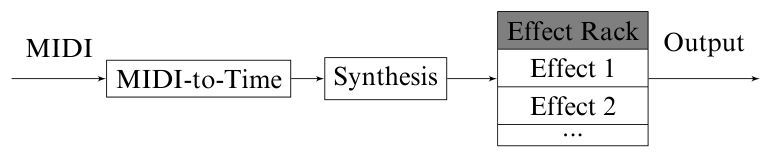
\includegraphics[width=\linewidth,height=.72\textheight,keepaspectratio]{assets/010_p003_vector1.png}\caption{Diagram or recorded result: Deliverables and assessment.}\label{fig:010_p003_vector10}\end{figure}
\clearpage
\section{Notes, rhythm, and MIDI timing}

MIDI describes musical events rather than recorded waveform samples. Equal temperament uses a frequency ratio of 2\textasciicircum{}(1/\allowbreak{}12) per semitone, with A4 =\allowbreak{} 440 Hz. For MIDI note n, f(n) =\allowbreak{} 440*2\textasciicircum{}((n-69)/\allowbreak{}12) Hz. Thus A3 =\allowbreak{} 220 Hz and A5 =\allowbreak{} 880 Hz. A periodic tone can contain harmonics at integer multiples of its fundamental;\allowbreak{} the fundamental need not be the largest spectral coefficient. The tables' MIDI CC heading refers here to note numbers, not control-change identifiers. Read note\_\allowbreak{}on and note\_\allowbreak{}off messages, channel, note number, velocity, and delta time. Channels share a common timeline and must be mixed rather than concatenated. A note\_\allowbreak{}on with zero velocity is ordinarily a note-off event. Pair events by channel and note and define a policy for repeated overlapping notes. Tempo is measured in microseconds per quarter note, and the file specifies ticks per quarter note. Convert delta ticks using the tempo active during that interval. The example tempo 576923, resolution 192 ticks/\allowbreak{}quarter, and duration 96 ticks give 288461.5 microseconds, approximately 0.288 seconds. A tempo change requires segment-wise conversion.

\begingroup\small\setlength{\tabcolsep}{3pt}\renewcommand{\arraystretch}{1.18}\begin{longtable}{@{}p{0.1171\linewidth}p{0.1171\linewidth}p{0.1171\linewidth}p{0.1171\linewidth}p{0.1171\linewidth}p{0.1171\linewidth}p{0.1171\linewidth}@{}}
\caption{Notes, rhythm, and MIDI timing - numerical data and parameters. (panel 1)}\label{tab:010_p004_table10}\\\toprule
\textbf{Note} & \textbf{Octave -1} & \textbf{Octave 0} & \textbf{Octave 1} & \textbf{Octave 2} & \textbf{Octave 3} & \textbf{Octave 4} \\ \midrule\endfirsthead \textbf{Note} & \textbf{Octave -1} & \textbf{Octave 0} & \textbf{Octave 1} & \textbf{Octave 2} & \textbf{Octave 3} & \textbf{Octave 4} \\ \midrule\endhead
C & 8.18 & 16.35 & 32.70 & 65.41 & 130.81 & 261.63 \\
C\#/\allowbreak{}Db & 8.66 & 17.32 & 34.65 & 69.30 & 138.59 & 277.18 \\
D & 9.18 & 18.35 & 36.71 & 73.42 & 146.83 & 293.66 \\
D\#/\allowbreak{}Eb & 9.72 & 19.45 & 38.89 & 77.78 & 155.56 & 311.13 \\
E & 10.30 & 20.60 & 41.20 & 82.41 & 164.81 & 329.63 \\
F & 10.91 & 21.83 & 43.65 & 87.31 & 174.61 & 349.23 \\
F\#/\allowbreak{}Gb & 11.56 & 23.12 & 46.25 & 92.50 & 185.00 & 369.99 \\
G & 12.25 & 24.50 & 49.00 & 98.00 & 196.00 & 392.00 \\
G\#/\allowbreak{}Ab & 12.98 & 25.96 & 51.91 & 103.83 & 207.65 & 415.30 \\
A & 13.75 & 27.50 & 55.00 & 110.00 & 220.00 & 440.00 \\
A\#/\allowbreak{}Bb & 14.57 & 29.14 & 58.27 & 116.54 & 233.08 & 466.16 \\
B & 15.43 & 30.87 & 61.74 & 123.47 & 246.94 & 493.88 \\
\bottomrule\end{longtable}\endgroup
\begingroup\small\setlength{\tabcolsep}{3pt}\renewcommand{\arraystretch}{1.18}\begin{longtable}{@{}p{0.1171\linewidth}p{0.1171\linewidth}p{0.1171\linewidth}p{0.1171\linewidth}p{0.1171\linewidth}p{0.1171\linewidth}p{0.1171\linewidth}@{}}
\caption{Notes, rhythm, and MIDI timing - numerical data and parameters. (panel 2)}\label{tab:010_p004_table11}\\\toprule
\textbf{Note} & \textbf{Octave 5} & \textbf{Octave 6} & \textbf{Octave 7} & \textbf{Octave 8} & \textbf{Octave 9} & \textbf{Octave 10} \\ \midrule\endfirsthead \textbf{Note} & \textbf{Octave 5} & \textbf{Octave 6} & \textbf{Octave 7} & \textbf{Octave 8} & \textbf{Octave 9} & \textbf{Octave 10} \\ \midrule\endhead
C & 523.25 & 1046.50 & 2093.00 & 4186.01 & 8372.02 & 16744.04 \\
C\#/\allowbreak{}Db & 554.37 & 1108.73 & 2217.46 & 4434.92 & 8869.84 & 17739.69 \\
D & 587.33 & 1174.66 & 2349.32 & 4698.64 & 9397.27 & 18794.55 \\
D\#/\allowbreak{}Eb & 622.25 & 1244.51 & 2489.02 & 4978.03 & 9956.06 & 19912.13 \\
E & 659.26 & 1318.51 & 2637.02 & 5274.04 & 10548.08 & 21096.16 \\
F & 698.46 & 1396.91 & 2793.83 & 5587.65 & 11175.30 & 22350.61 \\
F\#/\allowbreak{}Gb & 739.99 & 1479.98 & 2959.96 & 5919.91 & 11839.82 & 23679.64 \\
G & 783.99 & 1567.98 & 3135.96 & 6271.93 & 12543.85 & 25087.71 \\
G\#/\allowbreak{}Ab & 830.61 & 1661.22 & 3322.44 & 6644.88 & 13289.75 & 26579.50 \\
A & 880.00 & 1760.00 & 3520.00 & 7040.00 & 14080.00 & 28160.00 \\
A\#/\allowbreak{}Bb & 932.33 & 1864.66 & 3729.31 & 7458.62 & 14917.24 & 29834.48 \\
B & 987.77 & 1975.53 & 3951.07 & 7902.13 & 15804.27 & 31608.53 \\
\bottomrule\end{longtable}\endgroup
\begingroup\small\setlength{\tabcolsep}{3pt}\renewcommand{\arraystretch}{1.18}\begin{longtable}{@{}p{0.2200\linewidth}p{0.2200\linewidth}p{0.2200\linewidth}p{0.2200\linewidth}@{}}
\caption{Notes, rhythm, and MIDI timing - numerical data and parameters.}\label{tab:010_p004_table20}\\\toprule
\textbf{MIDI note number} & \textbf{Note name} & \textbf{Frequency (Hz)} & \textbf{Period (ms)} \\ \midrule\endfirsthead \textbf{MIDI note number} & \textbf{Note name} & \textbf{Frequency (Hz)} & \textbf{Period (ms)} \\ \midrule\endhead
21 & A0 & 27.50000 & 36.363636 \\
22 & A\#/\allowbreak{}Bb0 & 29.13524 & 34.322702 \\
23 & B0 & 30.86771 & 32.396317 \\
24 & C1 & 32.70320 & 30.578051 \\
25 & C\#/\allowbreak{}Db1 & 34.64783 & 28.861837 \\
26 & D1 & 36.70810 & 27.241947 \\
27 & D\#/\allowbreak{}Eb1 & 38.89087 & 25.712974 \\
28 & E1 & 41.20344 & 24.269816 \\
29 & F1 & 43.65353 & 22.907655 \\
30 & F\#/\allowbreak{}Gb1 & 46.24930 & 21.621948 \\
31 & G1 & 48.99943 & 20.408401 \\
32 & G\#/\allowbreak{}Ab1 & 51.91309 & 19.262965 \\
33 & A1 & 55.00000 & 18.181818 \\
34 & A\#/\allowbreak{}Bb1 & 58.27047 & 17.161351 \\
35 & B1 & 61.73541 & 16.198159 \\
36 & C2 & 65.40639 & 15.289026 \\
37 & C\#/\allowbreak{}Db2 & 69.29566 & 14.430919 \\
38 & D2 & 73.41619 & 13.620973 \\
39 & D\#/\allowbreak{}Eb2 & 77.78175 & 12.856487 \\
40 & E2 & 82.40689 & 12.134908 \\
41 & F2 & 87.30706 & 11.453828 \\
42 & F\#/\allowbreak{}Gb2 & 92.49861 & 10.810974 \\
43 & G2 & 97.99886 & 10.204200 \\
44 & G\#/\allowbreak{}Ab2 & 103.82617 & 9.631483 \\
45 & A2 & 110.00000 & 9.090909 \\
46 & A\#/\allowbreak{}Bb2 & 116.54094 & 8.580676 \\
47 & B2 & 123.47083 & 8.099079 \\
48 & C3 & 130.81278 & 7.644513 \\
49 & C\#/\allowbreak{}Db3 & 138.59132 & 7.215459 \\
50 & D3 & 146.83238 & 6.810487 \\
51 & D\#/\allowbreak{}Eb3 & 155.56349 & 6.428243 \\
52 & E3 & 164.81378 & 6.067454 \\
53 & F3 & 174.61412 & 5.726914 \\
54 & F\#/\allowbreak{}Gb3 & 184.99721 & 5.405487 \\
55 & G3 & 195.99772 & 5.102100 \\
56 & G\#/\allowbreak{}Ab3 & 207.65235 & 4.815741 \\
57 & A3 & 220.00000 & 4.545455 \\
58 & A\#/\allowbreak{}Bb3 & 233.08188 & 4.290338 \\
59 & B3 & 246.94165 & 4.049540 \\
60 & C4 & 261.62557 & 3.822256 \\
61 & C\#/\allowbreak{}Db4 & 277.18263 & 3.607730 \\
62 & D4 & 293.66477 & 3.405243 \\
63 & D\#/\allowbreak{}Eb4 & 311.12698 & 3.214122 \\
64 & E4 & 329.62756 & 3.033727 \\
65 & F4 & 349.22823 & 2.863457 \\
66 & F\#/\allowbreak{}Gb4 & 369.99442 & 2.702743 \\
67 & G4 & 391.99544 & 2.551050 \\
68 & G\#/\allowbreak{}Ab4 & 415.30470 & 2.407871 \\
69 & A4 & 440.00000 & 2.272727 \\
70 & A\#/\allowbreak{}Bb4 & 466.16376 & 2.145169 \\
71 & B4 & 493.88330 & 2.024770 \\
72 & C5 & 523.25113 & 1.911128 \\
73 & C\#/\allowbreak{}Db5 & 554.36526 & 1.803865 \\
74 & D5 & 587.32954 & 1.702622 \\
75 & D\#/\allowbreak{}Eb5 & 622.25397 & 1.607061 \\
\bottomrule\end{longtable}\endgroup
\begingroup\small\setlength{\tabcolsep}{3pt}\renewcommand{\arraystretch}{1.18}\begin{longtable}{@{}p{0.2200\linewidth}p{0.2200\linewidth}p{0.2200\linewidth}p{0.2200\linewidth}@{}}
\caption{Notes, rhythm, and MIDI timing - numerical data and parameters.}\label{tab:010_p005_table10}\\\toprule
\textbf{MIDI note number} & \textbf{Note name} & \textbf{Frequency (Hz)} & \textbf{Period (ms)} \\ \midrule\endfirsthead \textbf{MIDI note number} & \textbf{Note name} & \textbf{Frequency (Hz)} & \textbf{Period (ms)} \\ \midrule\endhead
76 & E5 & 659.25511 & 1.516863 \\
77 & F5 & 698.45646 & 1.431728 \\
78 & F\#/\allowbreak{}Gb5 & 739.98885 & 1.351372 \\
79 & G5 & 783.99087 & 1.275525 \\
80 & G\#/\allowbreak{}Ab5 & 830.60940 & 1.203935 \\
81 & A5 & 880.00000 & 1.136364 \\
82 & A\#/\allowbreak{}Bb5 & 932.32752 & 1.072584 \\
83 & B5 & 987.76660 & 1.012385 \\
84 & C6 & 1046.50226 & 0.955564 \\
85 & C\#/\allowbreak{}Db6 & 1108.73052 & 0.901932 \\
86 & D6 & 1174.65907 & 0.851311 \\
87 & D\#/\allowbreak{}Eb6 & 1244.50793 & 0.803530 \\
88 & E6 & 1318.51023 & 0.758432 \\
89 & F6 & 1396.91293 & 0.715864 \\
90 & F\#/\allowbreak{}Gb6 & 1479.97769 & 0.675686 \\
91 & G6 & 1567.98174 & 0.637763 \\
92 & G\#/\allowbreak{}Ab6 & 1661.21879 & 0.601968 \\
93 & A6 & 1760.00000 & 0.568182 \\
94 & A\#/\allowbreak{}Bb6 & 1864.65505 & 0.536292 \\
95 & B6 & 1975.53321 & 0.506192 \\
96 & C7 & 2093.00452 & 0.477782 \\
97 & C\#/\allowbreak{}Db7 & 2217.46105 & 0.450966 \\
98 & D7 & 2349.31814 & 0.425655 \\
99 & D\#/\allowbreak{}Eb7 & 2489.01587 & 0.401765 \\
100 & E7 & 2637.02046 & 0.379216 \\
101 & F7 & 2793.82585 & 0.357932 \\
102 & F\#/\allowbreak{}Gb7 & 2959.95538 & 0.337843 \\
103 & G7 & 3135.96349 & 0.318881 \\
104 & G\#/\allowbreak{}Ab7 & 3322.43758 & 0.300984 \\
105 & A7 & 3520.00000 & 0.284091 \\
106 & A\#/\allowbreak{}Bb7 & 3729.31009 & 0.268146 \\
107 & B7 & 3951.06641 & 0.253096 \\
108 & C8 & 4186.00904 & 0.238891 \\
109 & C\#/\allowbreak{}Db8 & 4434.92210 & 0.225483 \\
110 & D8 & 4698.63629 & 0.212828 \\
111 & D\#/\allowbreak{}Eb8 & 4978.03174 & 0.200883 \\
112 & E8 & 5274.04091 & 0.189608 \\
113 & F8 & 5587.65170 & 0.178966 \\
114 & F\#/\allowbreak{}Gb8 & 5919.91076 & 0.168921 \\
115 & G8 & 6271.92698 & 0.159441 \\
116 & G\#/\allowbreak{}Ab8 & 6644.87516 & 0.150492 \\
117 & A8 & 7040.00000 & 0.142045 \\
118 & A\#/\allowbreak{}Bb8 & 7458.62018 & 0.134073 \\
119 & B8 & 7902.13282 & 0.126548 \\
120 & C9 & 8372.01809 & 0.119446 \\
121 & C\#/\allowbreak{}Db9 & 8869.84419 & 0.112742 \\
122 & D9 & 9397.27257 & 0.106414 \\
123 & D\#/\allowbreak{}Eb9 & 9956.06348 & 0.100441 \\
124 & E9 & 10548.08182 & 0.094804 \\
125 & F9 & 11175.30341 & 0.089483 \\
126 & F\#/\allowbreak{}Gb9 & 11839.82153 & 0.084461 \\
127 & G9 & 12543.85395 & 0.079720 \\
\bottomrule\end{longtable}\endgroup
\begingroup\small\setlength{\tabcolsep}{3pt}\renewcommand{\arraystretch}{1.18}\begin{longtable}{@{}p{0.2200\linewidth}p{0.2200\linewidth}p{0.2200\linewidth}p{0.2200\linewidth}@{}}
\caption{Notes, rhythm, and MIDI timing - numerical data and parameters.}\label{tab:010_p006_table10}\\\toprule
\textbf{Message Type} & \textbf{Channel} & \textbf{Parameter} & \textbf{Time} \\ \midrule\endfirsthead \textbf{Message Type} & \textbf{Channel} & \textbf{Parameter} & \textbf{Time} \\ \midrule\endhead
program change
\_\allowbreak{} & 0 & program=\allowbreak{}71 & 0 \\
control change
\_\allowbreak{} & 0 & control=\allowbreak{}10, value=\allowbreak{}64 & 0 \\
note on
\_\allowbreak{} & 0 & note=\allowbreak{}73, velocity=\allowbreak{}96 & 0 \\
note off
\_\allowbreak{} & 0 & note=\allowbreak{}73, velocity=\allowbreak{}0 & 96 \\
note on
\_\allowbreak{} & 0 & note=\allowbreak{}83, velocity=\allowbreak{}96 & 0 \\
note off
\_\allowbreak{} & 0 & note=\allowbreak{}83, velocity=\allowbreak{}0 & 288 \\
note on
\_\allowbreak{} & 0 & note=\allowbreak{}80, velocity=\allowbreak{}96 & 0 \\
note off
\_\allowbreak{} & 0 & note=\allowbreak{}80, velocity=\allowbreak{}0 & 480 \\
note on
\_\allowbreak{} & 0 & note=\allowbreak{}78, velocity=\allowbreak{}96 & 0 \\
note on
\_\allowbreak{} & 0 & note=\allowbreak{}76, velocity=\allowbreak{}96 & 192 \\
note off
\_\allowbreak{} & 0 & note=\allowbreak{}78, velocity=\allowbreak{}0 & 0 \\
note off
\_\allowbreak{} & 0 & note=\allowbreak{}76, velocity=\allowbreak{}0 & 96 \\
note on
\_\allowbreak{} & 0 & note=\allowbreak{}75, velocity=\allowbreak{}96 & 0 \\
\bottomrule\end{longtable}\endgroup
\clearpage
\section{Oscillator synthesis}

The mandatory synthesis stage combines a periodic source with an amplitude envelope. Implement sine, sawtooth, triangle, and square waveforms. Parameters include waveform, phase, fundamental frequency, volume, and detuning;\allowbreak{} optional oscillator filtering uses a VCF. Phase and time delay are related for an individual sinusoid but are not interchangeable parameters for an arbitrary waveform. A Gaussian-noise source may be added;\allowbreak{} its amplitude is adjustable, but it has no unique fundamental or phase. Combine several oscillators as a weighted sum. Detuning uses nearby frequency offsets and weights:\allowbreak{} x\_\allowbreak{}detuned(t) =\allowbreak{} sum\_\allowbreak{}i A\_\allowbreak{}i*x(2*pi*(f\_\allowbreak{}b+\allowbreak{}f\_\allowbreak{}i)*t). The assignment permits a justified choice of oscillator count, offsets, and weights as functions of the detune control. Preserve amplitude headroom when mixing voices. Naively sampled nonsinusoidal waveforms can alias;\allowbreak{} discuss this limitation rather than treating every generated high harmonic as physically meaningful.

\begin{figure}[!htbp]\centering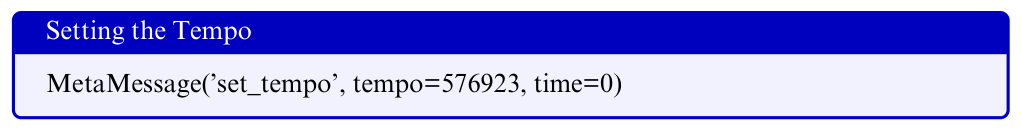
\includegraphics[width=\linewidth,height=.72\textheight,keepaspectratio]{assets/010_p007_vector1.png}\caption{Diagram or recorded result: Oscillator synthesis.}\label{fig:010_p007_vector10}\end{figure}
\clearpage
\section{AHDSR envelope}

Implement adjustable Attack, Hold, Decay, Sustain, and Release. Attack rises to peak, Hold stays at peak, Decay falls toward the sustain level, Sustain continues until note release, and Release falls to silence after note-off. Use exponential-like transitions as requested. A normalized exponential segment must have explicit endpoint behavior;\allowbreak{} the illustrative piecewise exponentials in the assignment should not be copied with discontinuities or without amplitude offsets. Support zero Hold and the specified zero-Sustain behavior. Velocity controls a documented amplitude mapping. Release must begin from the current envelope level when a short note ends before attack/\allowbreak{}decay has finished. Preserve the original envelope diagrams, including the exponential example.

\begin{figure}[!htbp]\centering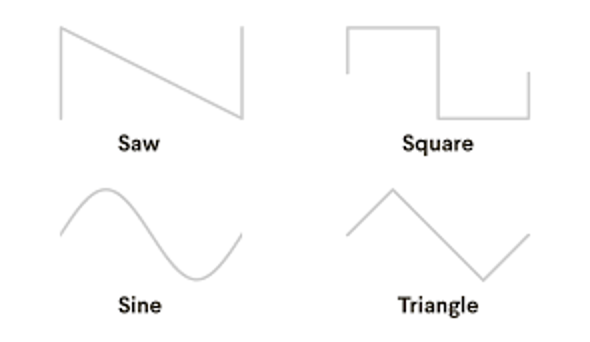
\includegraphics[width=\linewidth,height=.72\textheight,keepaspectratio]{assets/010_p010_01.png}\caption{Diagram or recorded result: AHDSR envelope.}\label{fig:010_p010_010}\end{figure}
\begin{figure}[!htbp]\centering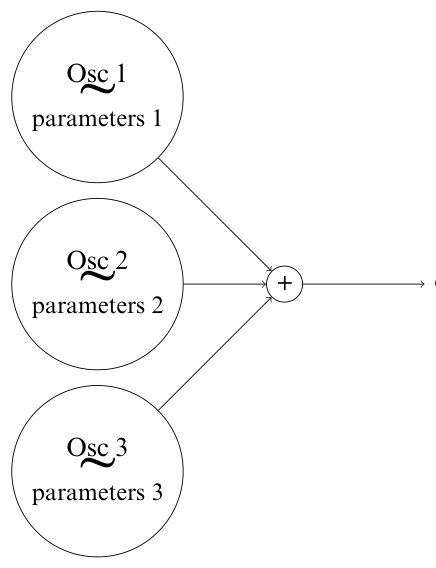
\includegraphics[width=\linewidth,height=.72\textheight,keepaspectratio]{assets/010_p010_vector1.png}\caption{Diagram or recorded result: AHDSR envelope.}\label{fig:010_p010_vector10}\end{figure}
\begin{figure}[!htbp]\centering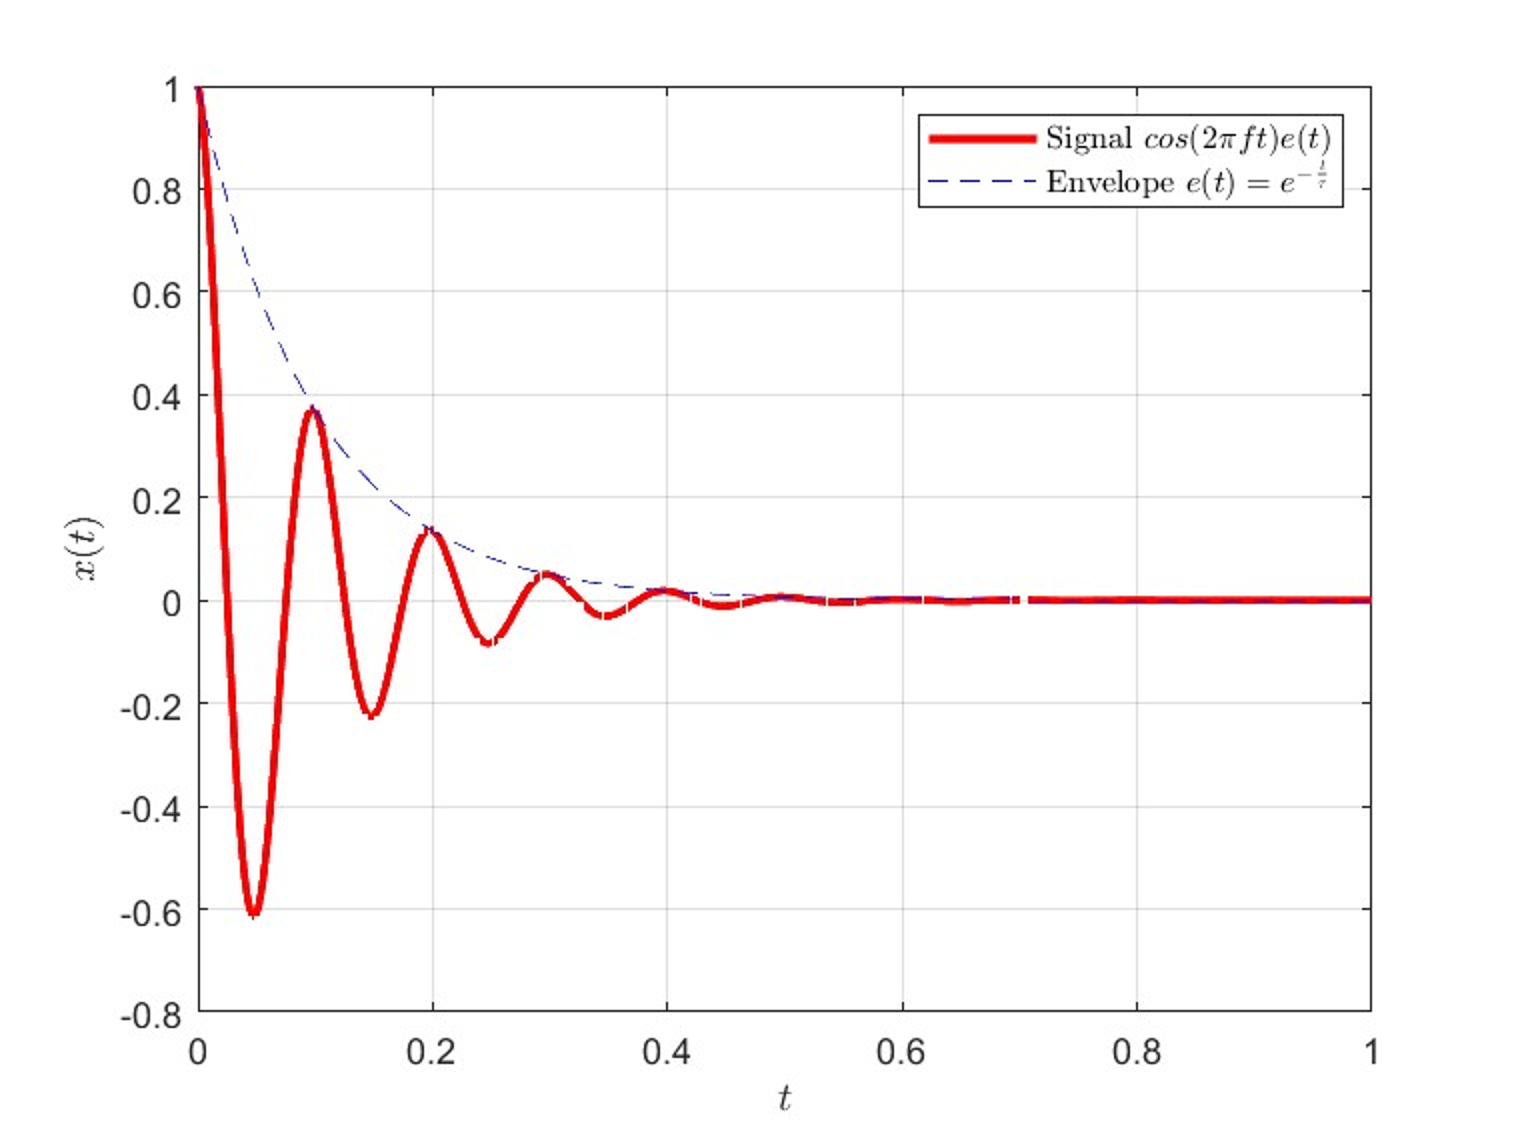
\includegraphics[width=\linewidth,height=.72\textheight,keepaspectratio]{assets/010_p012_01.png}\caption{Diagram or recorded result: AHDSR envelope.}\label{fig:010_p012_010}\end{figure}
\begin{figure}[!htbp]\centering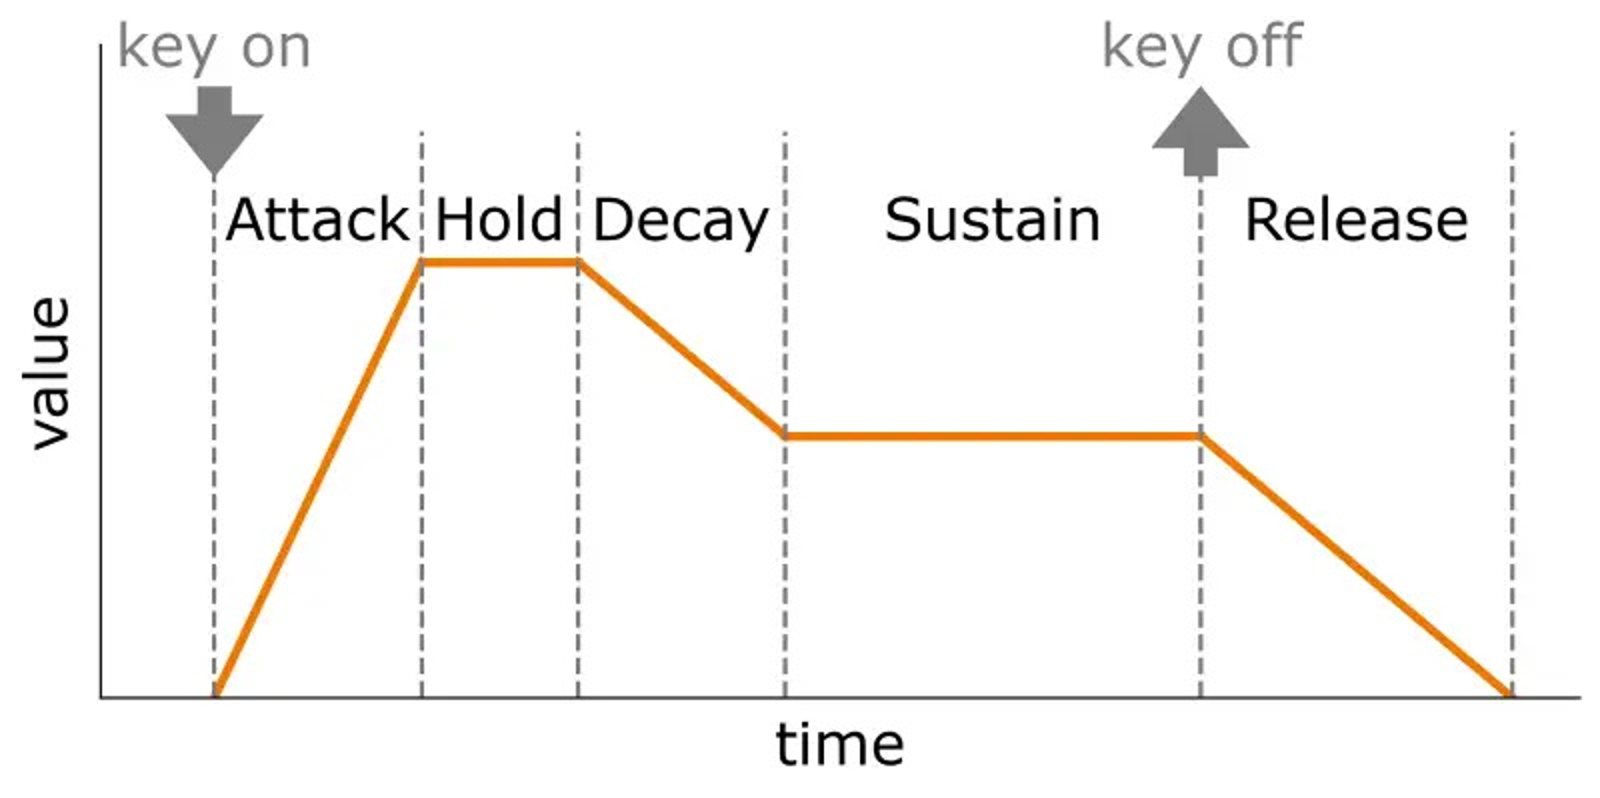
\includegraphics[width=\linewidth,height=.72\textheight,keepaspectratio]{assets/010_p012_02.png}\caption{Diagram or recorded result: AHDSR envelope.}\label{fig:010_p012_020}\end{figure}
\clearpage
\section{Shared effect interface}

An effect receives audio and returns transformed audio. A rack cascades several effects in an ordered chain. Every effect has input gain, output gain, and a wet/\allowbreak{}dry parameter w from zero to one;\allowbreak{} mix as (1-w)*dry +\allowbreak{} w*wet, with defined gain placement. Order matters for nonlinear effects. Expose parameters and sample rate rather than embedding unexplained constants.


\begingroup\small\setlength{\tabcolsep}{3pt}\renewcommand{\arraystretch}{1.2}
\begin{longtable}{@{}p{0.3100\linewidth}p{0.3100\linewidth}p{0.3100\linewidth}@{}}
\toprule
\textbf{Effect} & \textbf{Main points} & \textbf{Bonus points} \\ \midrule
\endfirsthead
\textbf{Effect} & \textbf{Main points} & \textbf{Bonus points} \\ \midrule \endhead
Phaser & 0.05 & 0.05 \\
Flanger & 0.05 & 0.05 \\
Chorus & 0.05 & 0.05 \\
Delay & 0.10 & 0.10 \\
Reverberation & 0.20 & none \\
Pitch shifter & 0.40 & none \\
Vocoder & 0.30 & none \\
Saturation & 0.25 & none \\
Compressor & 0.25 & none \\
Voltage-controlled filter & 0.10 & none \\
\bottomrule\end{longtable}\endgroup
\begin{figure}[!htbp]\centering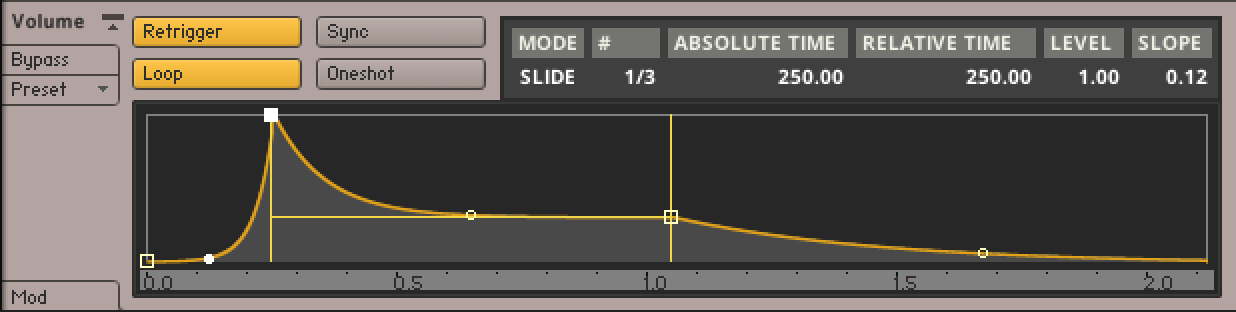
\includegraphics[width=\linewidth,height=.72\textheight,keepaspectratio]{assets/010_p013_01.png}\caption{Diagram or recorded result: Shared effect interface.}\label{fig:010_p013_010}\end{figure}
\begingroup\small\setlength{\tabcolsep}{3pt}\renewcommand{\arraystretch}{1.18}\begin{longtable}{@{}p{0.3000\linewidth}p{0.3000\linewidth}p{0.3000\linewidth}@{}}
\caption{Shared effect interface - numerical data and parameters.}\label{tab:010_p014_table10}\\\toprule
\textbf{Effect} & \textbf{Point} & \textbf{Bonus} \\ \midrule\endfirsthead \textbf{Effect} & \textbf{Point} & \textbf{Bonus} \\ \midrule\endhead
Phaser & 0.05 & 0.05 \\
Flanger & 0.05 & 0.05 \\
Chorus & 0.05 & 0.05 \\
Delay & 0.1 & 0.1 \\
Reverberation & 0.2 & - \\
Pitch Shifter & 0.4 & - \\
Vocoder & 0.3 & - \\
Saturation & 0.25 & - \\
Compressor & 0.25 & - \\
Voltage-Controlled Filter & 0.1 & - \\
\bottomrule\end{longtable}\endgroup
\clearpage
\section{Saturation and compression}

Implement hard clipping to [-T,T], soft clipping T*tanh(x/\allowbreak{}T), and the specified variable saturation T*abs(x/\allowbreak{}T)\textasciicircum{}a*sign(x). Drive D and bias b change the input to f(D*x+\allowbreak{}b). Define T > 0 and parameter ranges. This variable-power law is not necessarily a bounded clipper outside its intended range. Nonlinear processing can generate harmonics and aliasing. The compressor has threshold, ratio, attack, and release controls. Above a threshold in decibels, the steady-state level is T+\allowbreak{}(L-T)/\allowbreak{}R. Convert the resulting gain reduction back to a linear multiplier. Do not mix linear amplitudes with decibel thresholds or interpret a compression ratio as a fixed number of decibels. Use an appropriate level/\allowbreak{}envelope detector and discretize attack/\allowbreak{}release behavior. The source suggests averaging recent samples for smoother response;\allowbreak{} specify whether the detector uses magnitude, RMS, or another quantity.

\begin{figure}[!htbp]\centering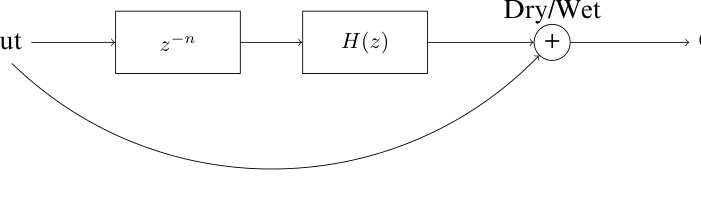
\includegraphics[width=\linewidth,height=.72\textheight,keepaspectratio]{assets/010_p017_vector1.png}\caption{Diagram or recorded result: Saturation and compression.}\label{fig:010_p017_vector10}\end{figure}
\clearpage
\section{Delay, phaser, flanger, and chorus}

Delay uses z\textasciicircum{}(-n) and an optional H(z) in the delayed branch. Convert time delay to samples using the sample rate. H(z)=\allowbreak{}1 gives the simple echo path;\allowbreak{} filtering or low-frequency modulation can add the stated extensions. Phaser mixes a dry signal with a cascade of all-pass-filter outputs. Phase differences produce frequency-dependent cancellation and peaks. Flanger uses a short delayed branch, optionally with feedback and modulation. Chorus uses multiple differently delayed/\allowbreak{}modulated branches to suggest several voices. Preserve the source diagrams and distinguish these related structures. The original typical-setting tables list phasing 0-3 ms with a little feedback, large modulation width, and slow speed;\allowbreak{} flanging 3-13 ms with substantial feedback and medium width/\allowbreak{}speed;\allowbreak{} chorus 13-30 ms with no feedback, small width, and medium speed. Earlier prose gives a 5-10 ms starting range for flanger/\allowbreak{}chorus. These are illustrative settings, not universal definitions. Optional LFO modulation applies to the three effects.

\begin{figure}[!htbp]\centering
\includegraphics[width=\linewidth,height=.72\textheight,keepaspectratio]{assets/010_p018_01.png}\caption{Diagram or recorded result: Delay, phaser, flanger, and chorus.}\label{fig:010_p018_010}\end{figure}
\begin{figure}[!htbp]\centering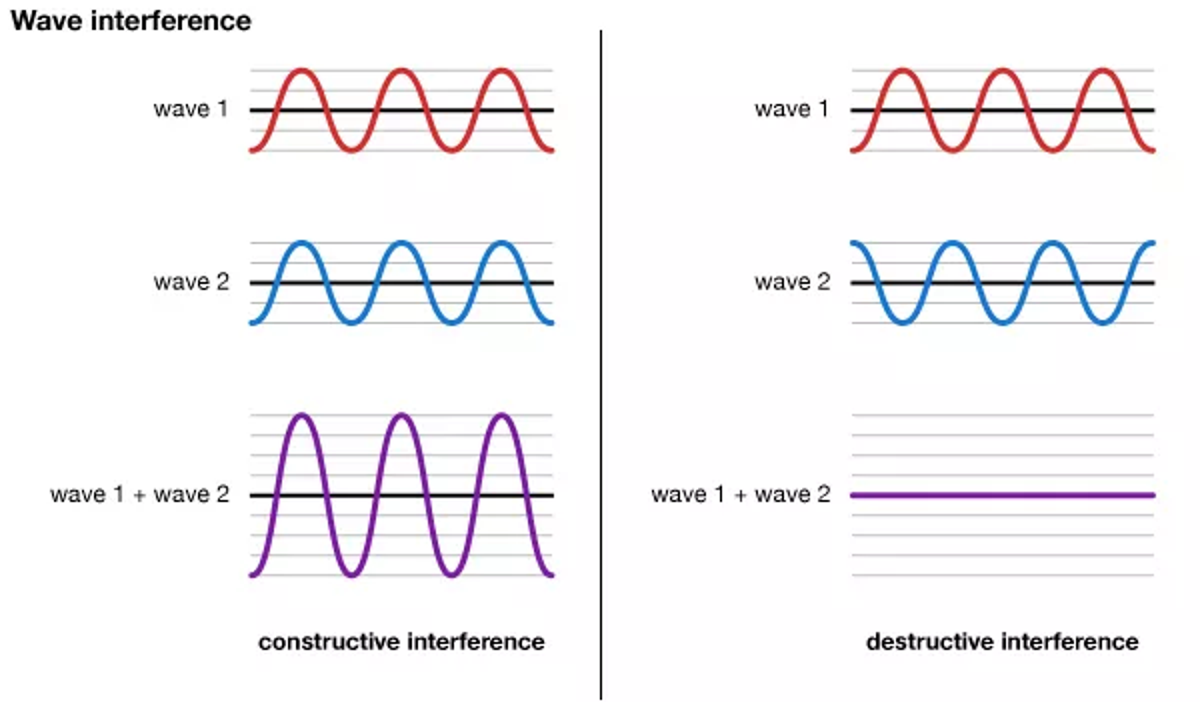
\includegraphics[width=\linewidth,height=.72\textheight,keepaspectratio]{assets/010_p018_02.png}\caption{Diagram or recorded result: Delay, phaser, flanger, and chorus.}\label{fig:010_p018_020}\end{figure}
\begin{figure}[!htbp]\centering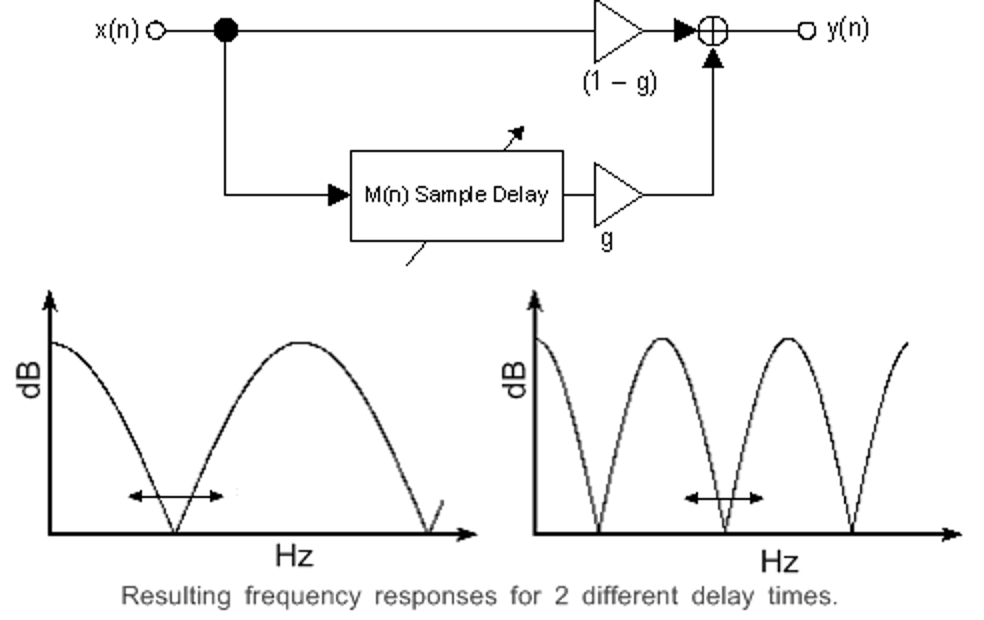
\includegraphics[width=\linewidth,height=.72\textheight,keepaspectratio]{assets/010_p019_01.png}\caption{Diagram or recorded result: Delay, phaser, flanger, and chorus.}\label{fig:010_p019_010}\end{figure}
\begingroup\small\setlength{\tabcolsep}{3pt}\renewcommand{\arraystretch}{1.18}\begin{longtable}{@{}p{0.1720\linewidth}p{0.1720\linewidth}p{0.1720\linewidth}p{0.1720\linewidth}p{0.1720\linewidth}@{}}
\caption{Delay, phaser, flanger, and chorus - numerical data and parameters.}\label{tab:010_p020_table10}\\\toprule
\textbf{Effect} & \textbf{Delay time} & \textbf{Feedback} & \textbf{Modulation} & \textbf{} \\ \midrule\endfirsthead \textbf{Effect} & \textbf{Delay time} & \textbf{Feedback} & \textbf{Modulation} & \textbf{} \\ \midrule\endhead
 &  &  & Width & Speed \\
Phasing & 0-3ms & A little & Lots & Slow \\
\bottomrule\end{longtable}\endgroup
\begingroup\small\setlength{\tabcolsep}{3pt}\renewcommand{\arraystretch}{1.18}\begin{longtable}{@{}p{0.1720\linewidth}p{0.1720\linewidth}p{0.1720\linewidth}p{0.1720\linewidth}p{0.1720\linewidth}@{}}
\caption{Delay, phaser, flanger, and chorus - numerical data and parameters.}\label{tab:010_p020_table20}\\\toprule
\textbf{Effect} & \textbf{Delay time} & \textbf{Feedback} & \textbf{Modulation} & \textbf{} \\ \midrule\endfirsthead \textbf{Effect} & \textbf{Delay time} & \textbf{Feedback} & \textbf{Modulation} & \textbf{} \\ \midrule\endhead
 &  &  & Width & Speed \\
Flanging & 3-13ms & Lots & Medium & Medium \\
\bottomrule\end{longtable}\endgroup
\begingroup\small\setlength{\tabcolsep}{3pt}\renewcommand{\arraystretch}{1.18}\begin{longtable}{@{}p{0.1720\linewidth}p{0.1720\linewidth}p{0.1720\linewidth}p{0.1720\linewidth}p{0.1720\linewidth}@{}}
\caption{Delay, phaser, flanger, and chorus - numerical data and parameters.}\label{tab:010_p020_table30}\\\toprule
\textbf{Effect} & \textbf{Delay time} & \textbf{Feedback} & \textbf{Modulation} & \textbf{} \\ \midrule\endfirsthead \textbf{Effect} & \textbf{Delay time} & \textbf{Feedback} & \textbf{Modulation} & \textbf{} \\ \midrule\endhead
 &  &  & Width & Speed \\
Chorus & 13-30ms & None & A little & Medium \\
\bottomrule\end{longtable}\endgroup
\clearpage
\section{Reverberation and filters}

Digital reverb can combine delayed branches with gains, using relatively prime delay lengths as suggested. A realistic sustained decay needs a defined network or sufficiently rich finite response;\allowbreak{} three isolated feedforward delays alone produce only a few echoes. Convolution reverb filters audio with a measured room impulse response. Match sample rates, manage output length, and document the impulse-response source. The VCF exposes low-pass, high-pass, band-pass, or band-stop behavior and adjustable cutoff. IIR implementations include direct forms I, II, and transposed structures. Keep coefficients and filter state separate. Direct form II stores internal state rather than merely a list of raw recent input samples. An LFO below approximately 20 Hz can vary oscillator frequency or filter cutoff. Recompute coefficients from a stable filter design;\allowbreak{} arbitrary coefficient perturbation may make poles unstable. Vibrato is frequency modulation and tremolo is amplitude modulation.

\begin{figure}[!htbp]\centering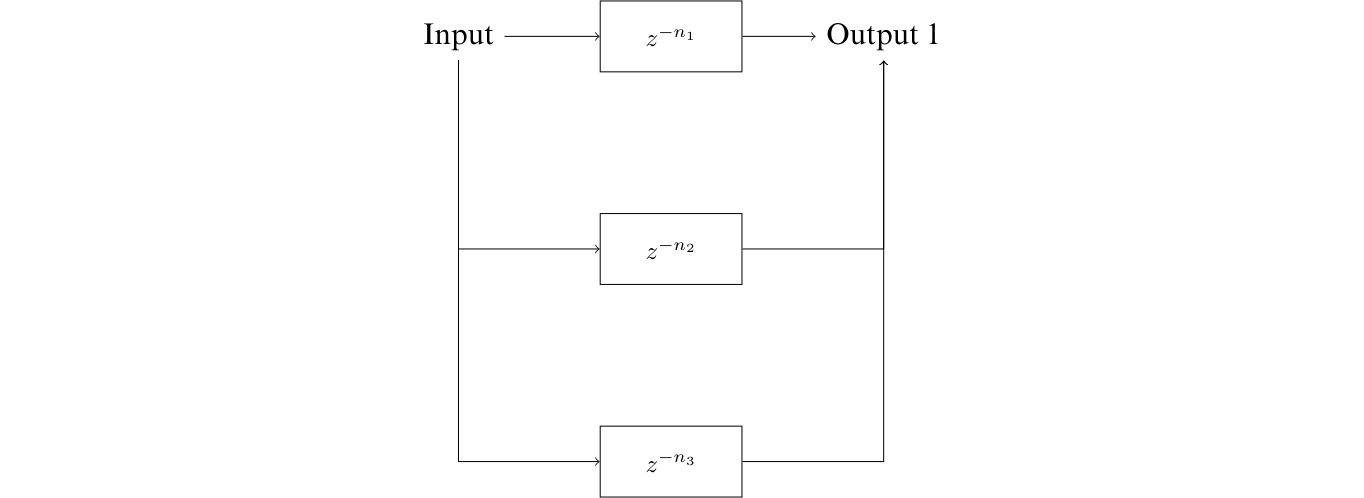
\includegraphics[width=\linewidth,height=.72\textheight,keepaspectratio]{assets/010_p021_diagram.png}\caption{Diagram or recorded result: Reverberation and filters.}\label{fig:010_p021_diagram0}\end{figure}
\begin{figure}[!htbp]\centering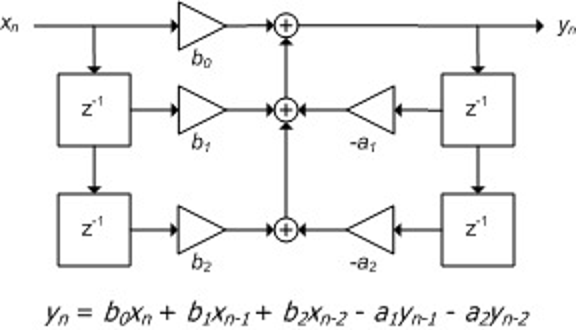
\includegraphics[width=\linewidth,height=.72\textheight,keepaspectratio]{assets/010_p022_01.png}\caption{Diagram or recorded result: Reverberation and filters.}\label{fig:010_p022_010}\end{figure}
\begin{figure}[!htbp]\centering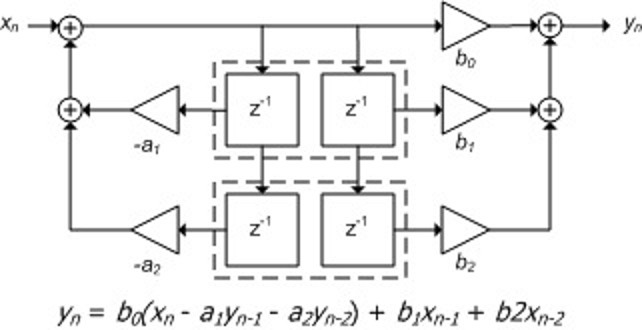
\includegraphics[width=\linewidth,height=.72\textheight,keepaspectratio]{assets/010_p022_02.png}\caption{Diagram or recorded result: Reverberation and filters.}\label{fig:010_p022_020}\end{figure}
\clearpage
\section{Vocoder and pitch shifting}

For the vocoder, divide the useful spectrum into logarithmically spaced bands, filter the carrier and speech modulator in each band, estimate modulator envelopes, apply each envelope to its carrier band, and sum. The assignment gives y[n] =\allowbreak{} sum\_\allowbreak{}i abs(m\_\allowbreak{}i[n])*c\_\allowbreak{}i[n];\allowbreak{} practical smoothing of the rectified envelope improves behavior. Use roughly a dozen or more bands, stable filters, and a useful lower frequency bound. Preserve carrier duration by padding or truncating the modulator. For pitch shifting, a three-semitone shift maps C-sharp4 to E4 and uses frequency ratio 2\textasciicircum{}(3/\allowbreak{}12), not a literal ratio of three. Simple resampling changes duration. The proposed phase-vocoder method first changes time scale without changing pitch, then resamples to restore duration. Analysis uses STFT, processing tracks/\allowbreak{}corrects phase with optional phase locking, and synthesis uses inverse STFT and overlap-add with compatible windows/\allowbreak{}hops. Preserve the original phase-vocoder diagram and explain the chosen implementation's artifacts and limits.

\begin{figure}[!htbp]\centering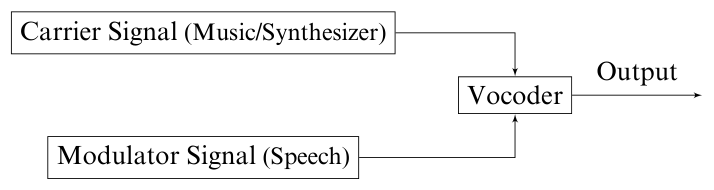
\includegraphics[width=\linewidth,height=.72\textheight,keepaspectratio]{assets/010_p024_vector1.png}\caption{Diagram or recorded result: Vocoder and pitch shifting.}\label{fig:010_p024_vector10}\end{figure}
\begin{figure}[!htbp]\centering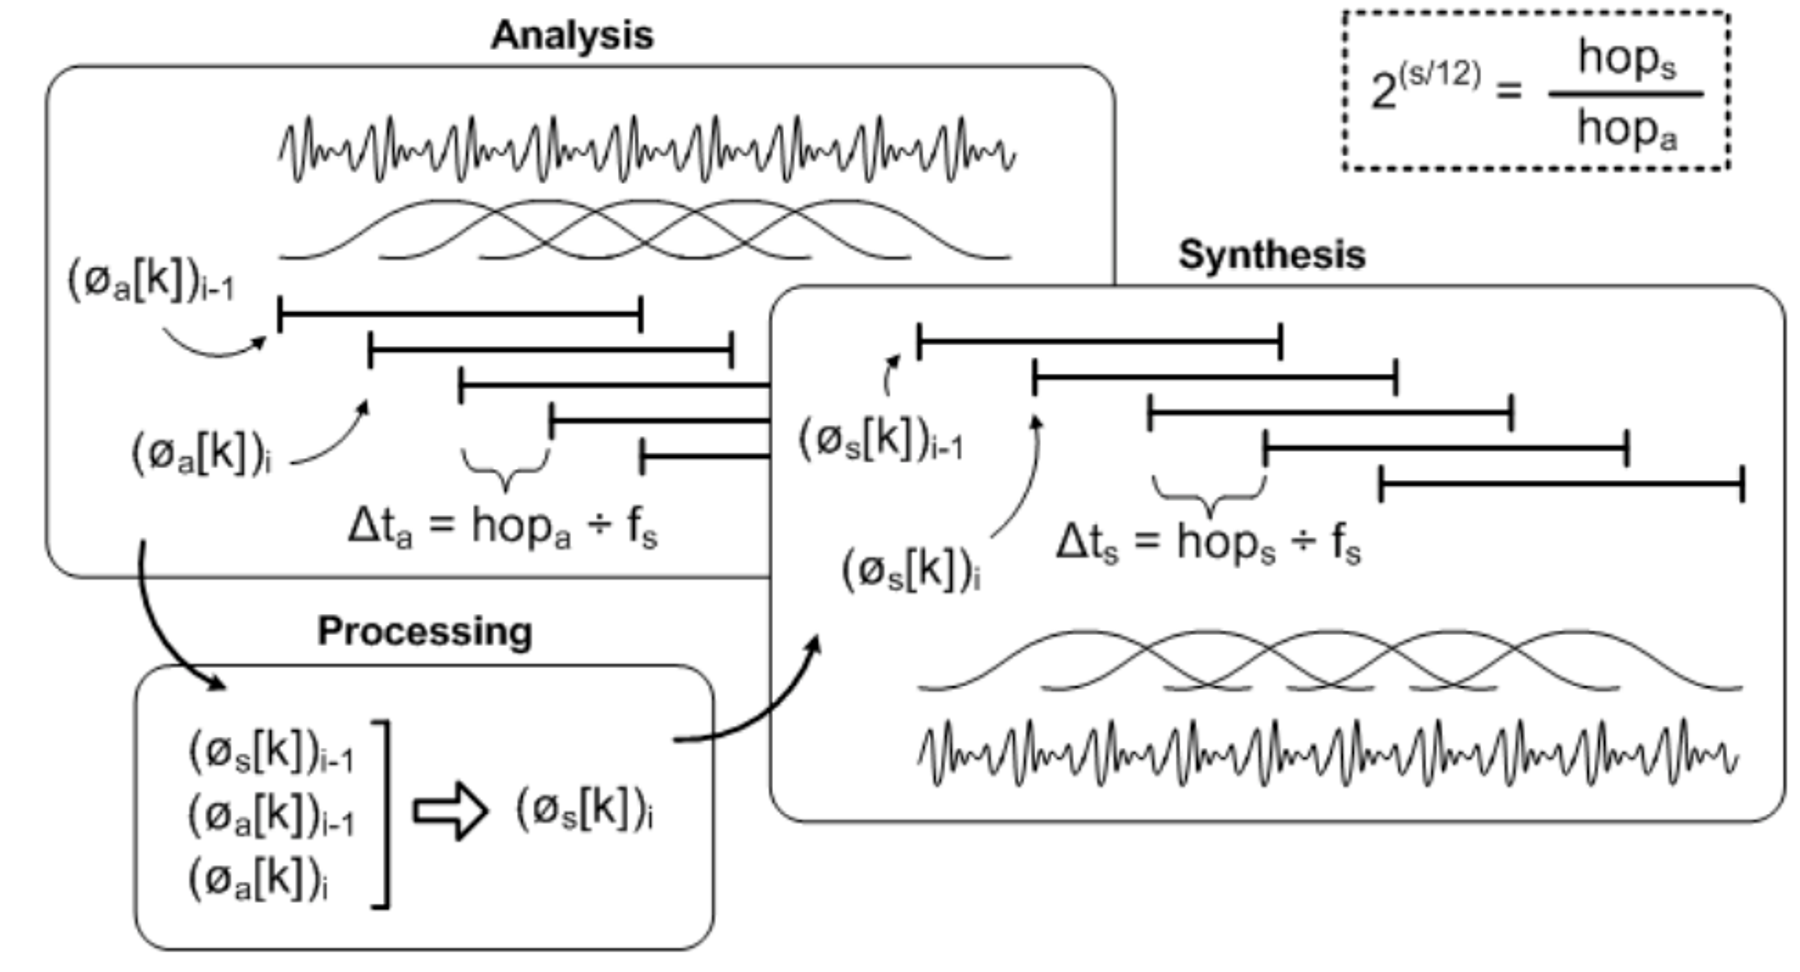
\includegraphics[width=\linewidth,height=.72\textheight,keepaspectratio]{assets/010_p025_01.png}\caption{Diagram or recorded result: Vocoder and pitch shifting.}\label{fig:010_p025_010}\end{figure}
\clearpage
\end{document}